\documentclass{beamer}
\setbeamertemplate{navigation symbols}{}


%\usepackage[numberedbib]{apacite}
%\bibliographystyle{plain}
\bibliographystyle{unsrt}
%\usepackage{natbib}
\usepackage{notoccite}

\usepackage{beamerthemeshadow}
\setbeamertemplate{caption}[numbered]

\hypersetup{colorlinks}

\def\gw#1{gravitational wave#1 (GW#1)\gdef\gw{GW}}
\def\gwb#1{gravitational wave burst#1 (GWB#1)\gdef\gw{GWB}}
\def\ns#1{neutron star#1 (NS#1)\gdef\ns{NS}}

\newcommand{\red}[1]{{\color{red}{#1}}}

\setbeamertemplate{bibliography item}[text]

\begin{document}
\title{}
\subtitle{Gravitational Wave Bursts: Inferences Without (Many) Assumptions}  
\author{James A. Clark}
%\institute{Georgia Institute Of Technology}

\date{\today} 

\begin{frame}[plain]
\titlepage
\begin{figure}
    \centering
    \scalebox{0.5}{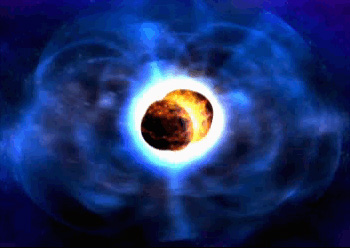
\includegraphics{title_magnetar.png}}
\end{figure}
\end{frame}

\begin{frame}
    \frametitle{Outline}
    \tableofcontents
\end{frame} 

%\section{Me}

%\begin{frame}
%    \frametitle{Background \& Interests}
%    \begin{itemize}
%        \item
%    \end{itemize}
%\end{frame}

\section{My Research}
\begin{frame}
    \frametitle{Current / past work}
    Highlights:
    \begin{itemize}
        \item Electromagnetically-triggered searches for transient \gw{s} in LIGO data.
            E.g.,
            \begin{itemize}
                \item Neutron star $f$-mode oscillations associated with pulsar
                    glitches~\cite{s5velaglitch-paper}
                \item Searches for un-modelled GW bursts \& inspiral signals
                    associated with
                    GRBs~\cite{2012arXiv1201.4413T,0004-637X-760-1-12}
            \end{itemize}
        \item Prospects for \dots
            \begin{itemize}
                \item \dots ``joint gravitational wave and short gamma-ray burst
                    observations''~\cite{2014arXiv1409.8149C}
                \item \dots \red{``high frequency burst searches following binary
                    neutron star coalescence with advanced gravitational wave
                detectors''}~\cite{clark:14}
            \end{itemize}
    \end{itemize}

        Generally, violent events in neutron stars, Bayesian inference \&
    machine learning $\leftrightarrow$ astrophysical inference from \gwb{s}

\end{frame}

\section{Gravitational Wave `Bursts'}

%\begin{frame}
%    \tableofcontents[currentsection]
%\end{frame}


%\subsection{Source Classes}
\begin{frame}
    \frametitle{GW Sources \& Ground-based Detectors}
    \begin{itemize}
        \item \dots
    \end{itemize}
\end{frame}

\subsection{Burst Analysis Strategies}
\begin{frame}
    \frametitle{Gravitational Wave ``Bursts''}

    \begin{columns}[]
        \column{0.5\textwidth}
        \begin{itemize}
            \item Transient: duration $\sim \mathcal{O}(10^{-3}-100)$\,s
            \item Uncertain morphology: matched-filtering ineffective or biased
            \item More certain morphology but few waveform cycles: `excess
                power' searches competitive with matched-filtering
        \end{itemize}

        \column{0.5\textwidth}
        \vspace{-1cm}
        \begin{figure}
            \centering
            \scalebox{0.18}{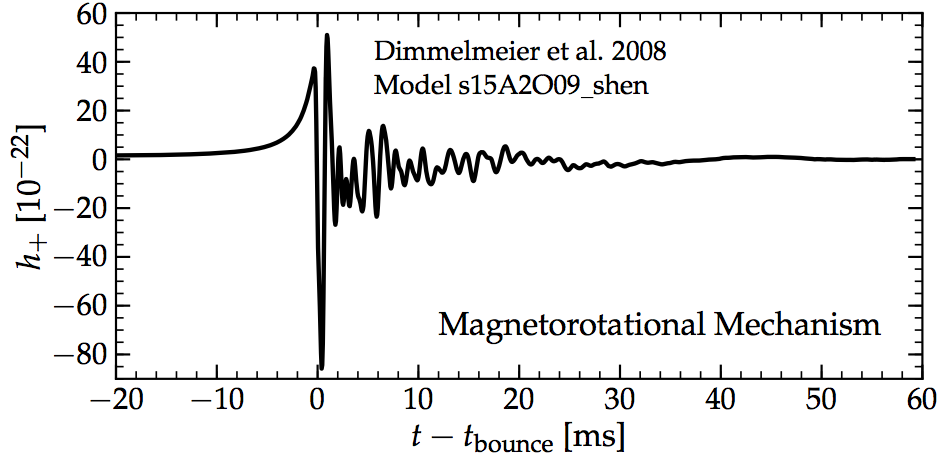
\includegraphics{sne_example.png}} \\
            \scalebox{0.44}{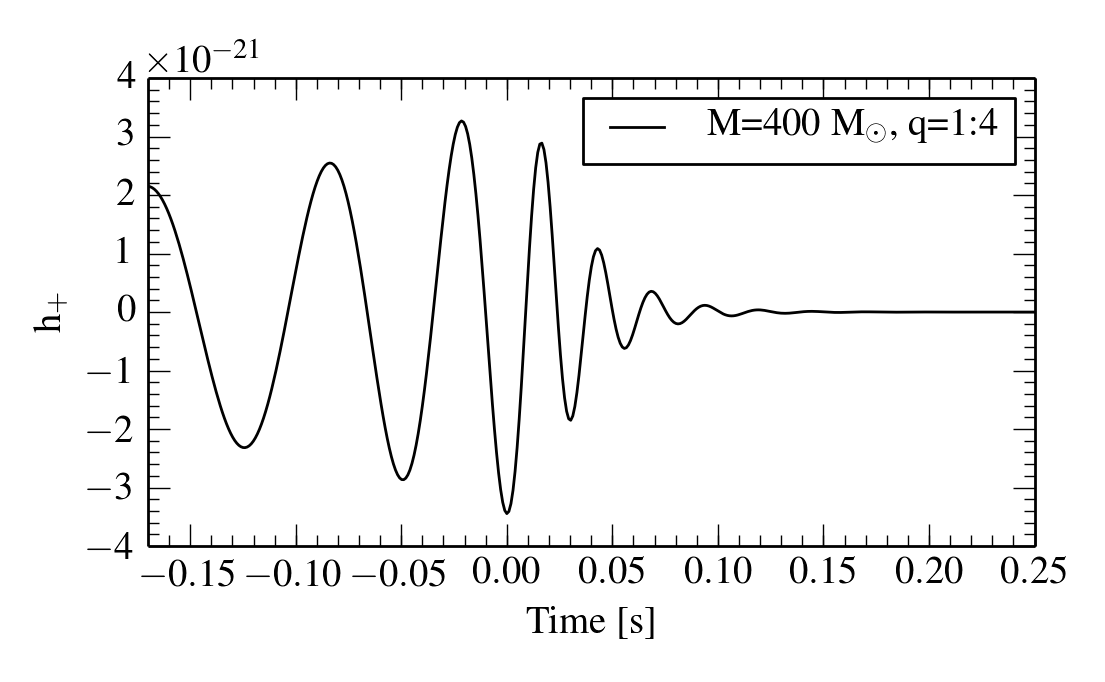
\includegraphics{imbbh_example.png}}
%            \scalebox{0.4}{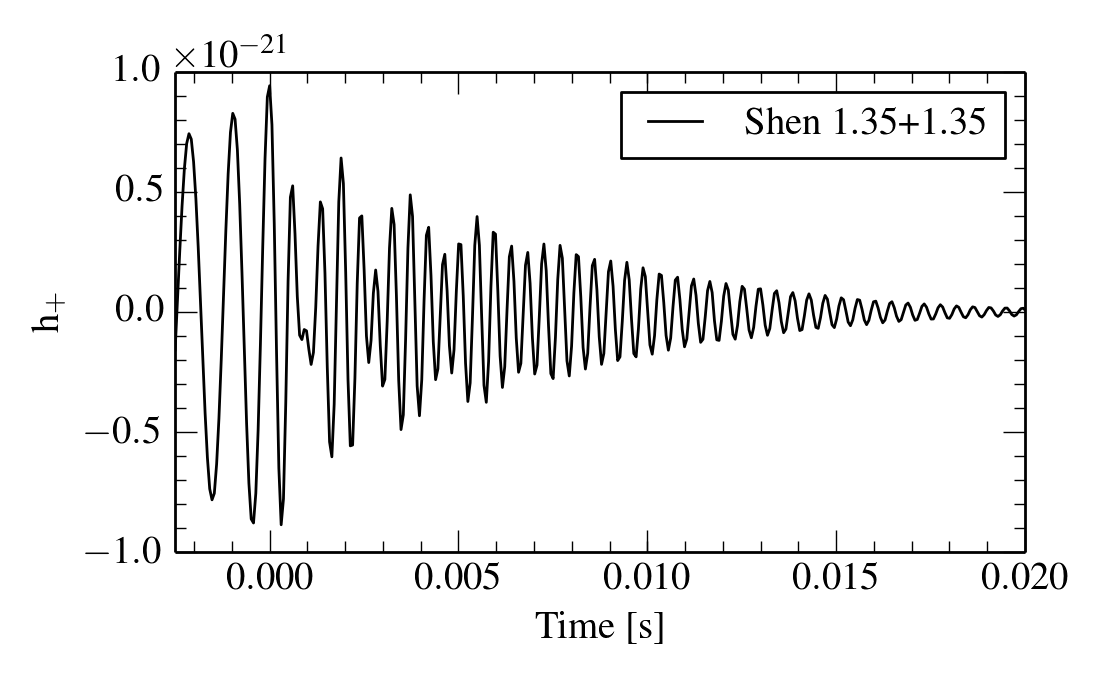
\includegraphics{pmns_example.png}}
        \end{figure}

    \end{columns}

\end{frame}

\begin{frame}
    \frametitle{GWB Analysis: Excess Power}
    \begin{itemize}
        \item Time-frequency decomposition of detector time-series data 
        \item `Excess power' due to e.g., GWs manifests as hot pixels in
            time-frequency plane
    \end{itemize}

    \begin{columns}[]
        \column{0.5\textwidth}
        \begin{figure}
            \scalebox{0.25}{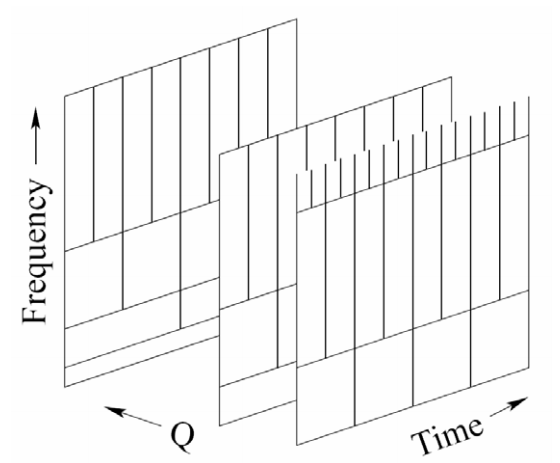
\includegraphics{multi_res_tf_cartoon.png}}
        \end{figure}
        \column{0.5\textwidth}
        \begin{block}{Time-Frequency Analysis}
            Typically decompose data at multiple resolutions via e.g., wavelets
            , Q-transforms, STFTs%: high time-resolution at
            %high-frequencies; high-frequency
            %resolution at low frequencies
        \end{block}
    \end{columns}

\end{frame}

\begin{frame}
    \frametitle{GWB Analysis: Excess Power}
    Example: binary neutron star inspiral signal observed in Hanford and
    Livingston detectors (blind hardware injection during final science run)
    
%   \begin{columns}[h]
%       \column{0.5\textwidth}
        \begin{figure}
            \centering
            \scalebox{0.5}{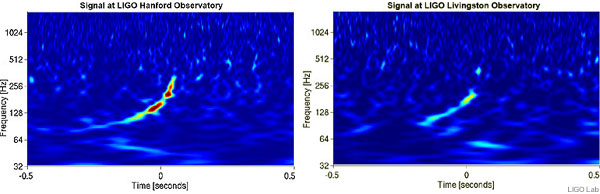
\includegraphics{bigdog.jpg}}
        \end{figure}
%    \end{columns}
\end{frame}

\begin{frame}
    \frametitle{GWBs: Coherent Analysis}
    \begin{itemize}
        \item {\bf Problem:} GW detector data: highly-nonstationary, \emph{full}
            of excess power
        \item {\bf Solution:} search for \emph{coherent} power a detector
            network
    \end{itemize}
    Single-pixel network analysis (following e.g.,~\cite{XP}):
    \begin{equation}
        \underbrace{
    \left[ \begin{array}
    {c} d_1 \\ d_2  \\ \vdots \\ d_D
    \end{array} \right]}_{\text{measured data}} = 
    \underbrace{\begin{bmatrix} 
            F_1^{+}(\mathbf{\Omega})/\sigma_1 & F_1^{\times}(\mathbf{\Omega})/\sigma_1 \\ 
            F_2^{+}(\mathbf{\Omega})/\sigma_2 & F_2^{\times}(\mathbf{\Omega})/\sigma_2 \\ 
            \vdots & \vdots \\ 
            F_D^{+}(\mathbf{\Omega})/\sigma_D & F_D^{\times}(\mathbf{\Omega})/\sigma_D  
    \end{bmatrix} }_{\text{whitened antenna responses}}
\underbrace{\left[ \begin{array}{c} h_+ \\ h_{\times} \end{array}
    \right]}_{\text{GW polarizations}}
+ \underbrace{\left[ \begin{array}{c} n_1 \\ n_2 \\ \vdots \\ n_D \end{array}
    \right]}_{\text{noise}}
\end{equation}
%
i.e.,
\begin{eqnarray}
    \mathbf{d} & = &\left[\mathbf{F}_+ \mathbf{F}_{\times}\right]\mathbf{h} +
    \mathbf{n} \nonumber \\
    & = & \mathbf{F}\mathbf{h} + \mathbf{n}
\end{eqnarray}


\end{frame}

\begin{frame}
    \frametitle{GWBs: Coherent Analysis}

    Likelihood for signal ($h$) vs noise (0):
    \begin{equation}
        \mathcal{L} = 2 \log
        \frac{P(\mathbf{d}|\mathbf{h})}{P(\mathbf{d}|0)} = |\mathbf{d}|^2  - |\mathbf{d} -
        \mathbf{F}\mathbf{h}|^2
    \end{equation}

    \begin{itemize}
%        \item Best-fit waveform $\hat{\mathbf{h}}$ maximises $\mathcal{L}$:
%            \begin{equation}
%                0 = \frac{\partial \mathcal{L}}{\partial h}\bigg\rvert_{h=\hat{h}}
%            \end{equation}
        %\item But no signal model for $h$?
        \item Treat waveform values $\mathbf{h} = (h_+,~h_{\times})$ in each
            pixel as free parameters; maximise $\mathcal{L}$ to form
            \emph{standard likelihood}
            \begin{equation}
                E_{\text{SL}} = \mathbf{d}^{T} \mathbf{F} \mathbf{F}_{\text{MP}}^{-1} \mathbf{d}
            \end{equation}
        \item where $\mathbf{F}_{\text{MP}}^{-1} = (\mathbf{F}^T\mathbf{F})^{-1}\mathbf{F}^T$
        \item $\mathbf{F}\mathbf{F}_{\text{MP}}^{-1}$ projects data onto
            $(\mathbf{F_+,F_{\times}})$ sub-space
        \item Residual data with signal removed should be Gaussian.  Can reject
            non-Gaussian glitches by looking at the null energy:
            \begin{equation}
                E_{\text{null}} =
                \mathbf{d}^{T}(\mathbf{I}-\mathbf{F}\mathbf{F}_{\text{MP}}^{-1})\mathbf{d}
            \end{equation}

    \end{itemize}

%   \begin{columns}[]
%       \column{0.5\textwidth}
%       \vspace{-1cm}
%       \begin{center}
%       \begin{figure}
%           \scalebox{0.25}{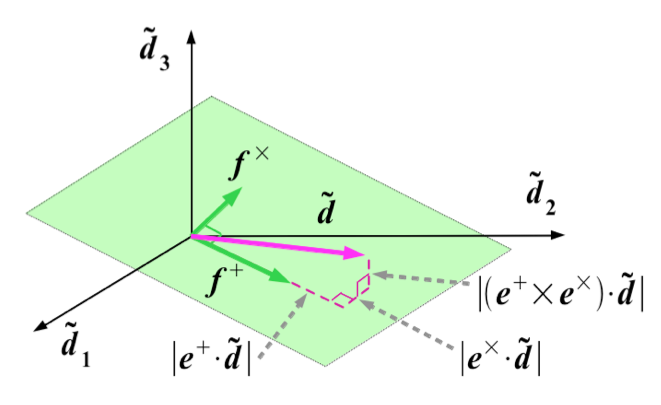
\includegraphics{projections.png}}
%       \end{figure}
%       \end{center}
%
%       \column{0.5\textwidth}
%       \begin{itemize}
%           \item Data: D-dimensional space
%           \item $(\mathbf{F_+,F_{\times}})$
%           \item Generally work in \emph{dominant polarization frame}
%           \item 
%       \end{itemize}
%   \end{columns}

\end{frame}

%\begin{frame}
%    \frametitle{GWBs: Coherent Analysis}
%    \begin{itemize}
%        \item \dots
%    \end{itemize}
%\end{frame}
%
%\begin{frame}
%    \frametitle{Coherent Analysis \& Glitch Rejection}
%    \begin{itemize}
%        \item \dots
%    \end{itemize}
%\end{frame}

\subsection{Burst Analysis Example: Binary Neutron Star Coalescence}

%\subsubsection{Binary Neutron Star Mergers}

\begin{frame}
    \tableofcontents[currentsection]
\end{frame}


\begin{frame}
    \frametitle{Binary Neutron Star Mergers \& GWBs}
    \begin{columns}[]
        \column{0.6\textwidth}
        \begin{center}

            \begin{small}
                \begin{itemize}
                    \item BNS \emph{inspiral} detectable to 200\,Mpc in
                        aLIGO\footnotemark
                    \item Post-merger scenarios:
                        \begin{enumerate}
                            \item prompt-collapse
                            \item quasi-stable NS
                            \item stable NS
                        \end{enumerate}
                    \item 2, 3 favored by many simulations, equations of state
                    \item GW morphology poorly known, broadband power in $\sim
                        1-4$\,kHz + dominant oscillation frequency
                    \item Detectable to few--10's\,Mpc

                \end{itemize}
            \end{small}

    \end{center}


        \column{0.5\textwidth}

    \begin{center}
        \vspace{-0.75cm}
        \begin{figure}
            \scalebox{0.35}{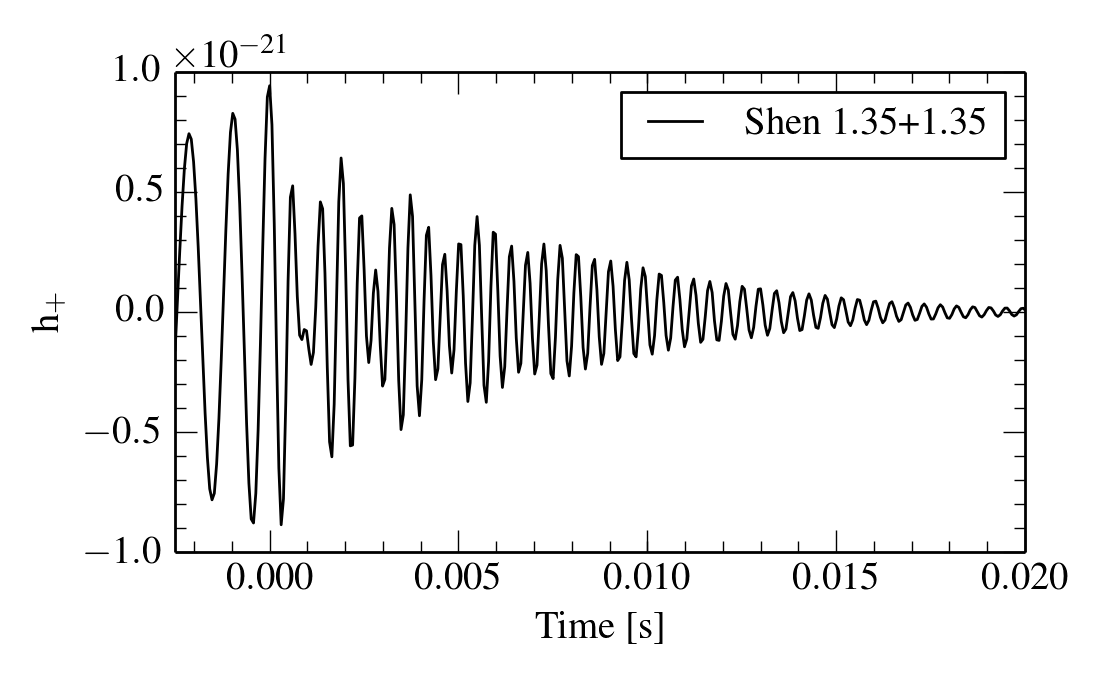
\includegraphics{pmns_example.png}} \\
            \scalebox{0.25}{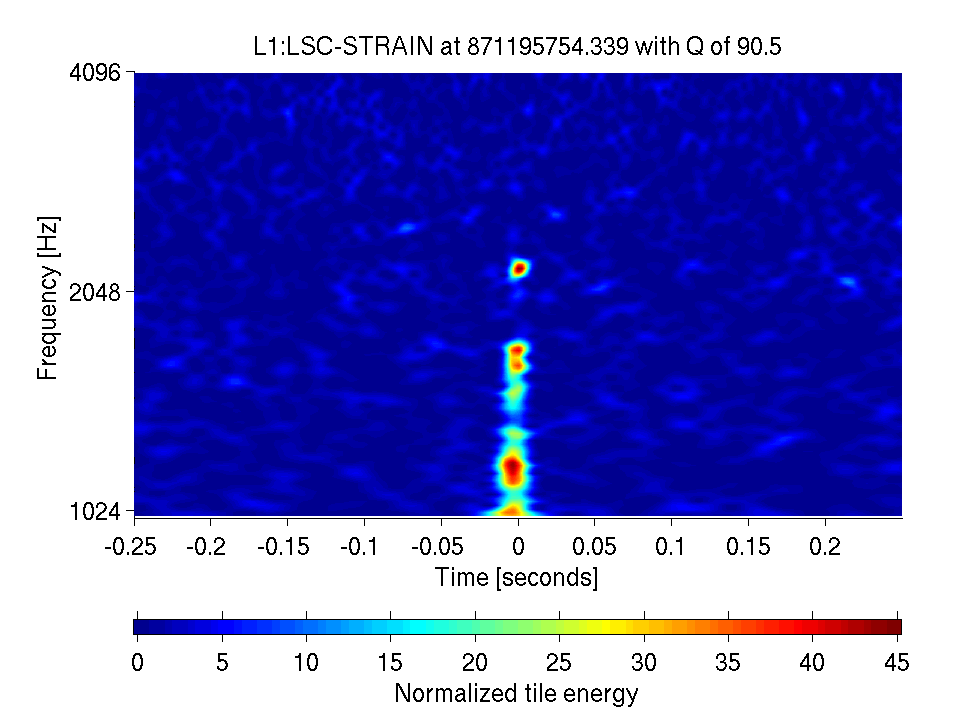
\includegraphics{pmns_tfmap.png}}
        \end{figure}

    \end{center}

    \end{columns}
    \footnotetext[1]{\tiny{at design sensitivity $\sim 2019$}}

\end{frame}

\begin{frame}
    \frametitle{Post-merger Oscillations \& NS EOS}
    \begin{small}
    \begin{itemize}
        \item Bauswein et al~\cite{Bauswein38Eos}: dominant post-merger
            oscillation frequency ($f_{\text{peak}}$) correlates with fiducial NS radius
        \item Takami et al~\cite{2014PhRvL.113i1104T}: similar findings +
            possible correlation of sub-dominant freq. with NS compactness
        \item Bauswein et al~\cite{2013PhRvL.111m1101B}: constrain maximimum NS
            mass with $f_{\text{peak}}$
    \end{itemize}
    \begin{columns}[]
        \column{0.2\textwidth}
        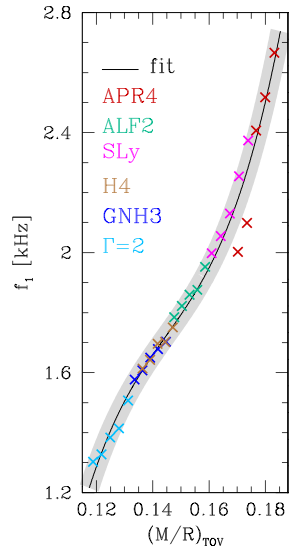
\includegraphics[width=\textwidth]{takami_compactness.png} \\
        \centering
        \tiny{Takami et al: $f_1-M/R$ correlation}
        \column{0.45\textwidth}
        \vspace{-0.35cm}
        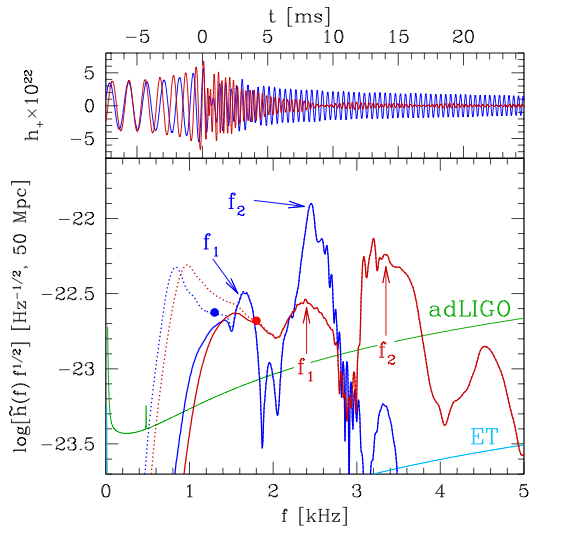
\includegraphics[width=\textwidth]{takami_spectrum.png} \\
        %\tiny{Takami et al: Time series \& spectra}
        \column{0.36\textwidth}
        \centering
        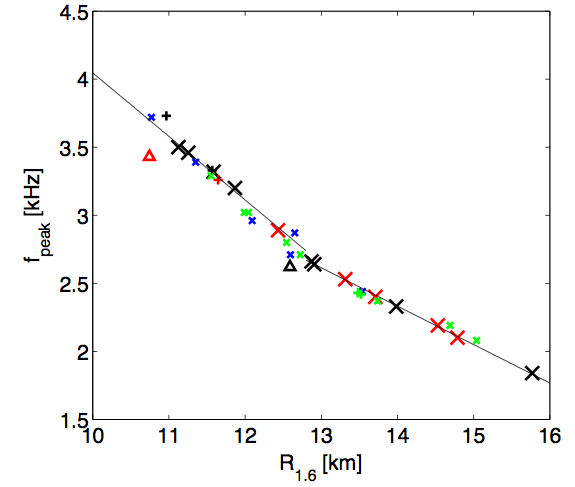
\includegraphics[width=\textwidth]{bauswein_fpeak.png} \\
        \tiny{Bauswein et al: $f_{\text{peak}}-R_{1.6}$ correlation}
    \end{columns}
\end{small}
\end{frame}

\begin{frame}
    \frametitle{Measuring Post-merger Oscillations In GWs}
    Clark et al~\cite{clark:14}: developed algorithm to analyze post-merger
    signatures detected (and reconstructed) by burst searches.\\
    Basic idea:
    \begin{itemize}
        \item Search for statistically significant, high-frequenccy power at
            time around BNS coalescence
        \item Detection $\rightarrow$ reconstructs signal $\hat{\mathbf{h}}$
        \item Spectral analysis of $\hat{\mathbf{h}}$ allows classification of
            prompt/delayed collapse, measurement of $f_{\text{peak}}$
    \end{itemize}
    Allows to detect signal and extract astrophysically relevant information
    without precise waveform models, just generic features ($f_{\text{peak}}$)
\end{frame}

\begin{frame}

    \frametitle{Measuring Post-merger Oscillations In GWs}

    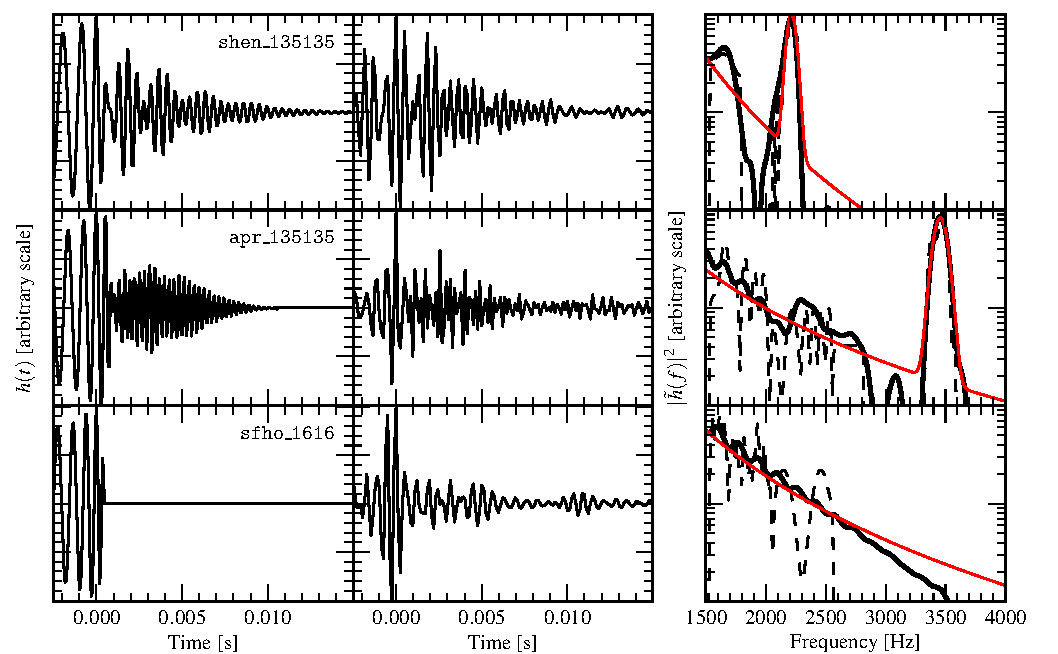
\includegraphics[width=\textwidth]{example_reconstruction.pdf}

\end{frame}

\begin{frame}
    \frametitle{Measuring Post-merger Oscillations In GWs}
    \begin{columns}[]
        \column{0.6\textwidth}
        \centering
        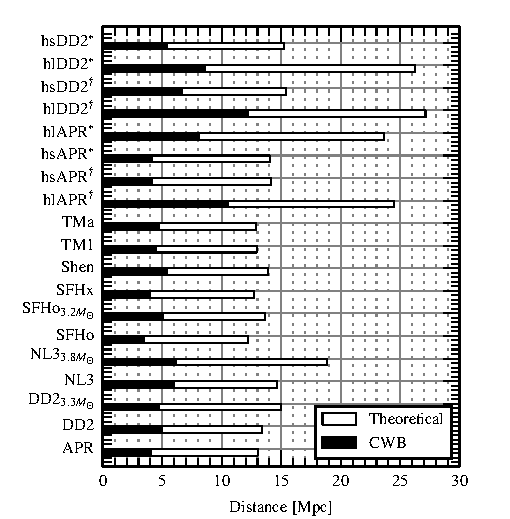
\includegraphics[width=\textwidth]{distances.pdf}

    \column{0.5\textwidth}
    {\small
        \begin{itemize}
            \item Compared theoretical matched-filter \& \emph{realistic} burst
                search detectability for aLIGO network for different EoSs
            \item Translate $f_{\text{peak}}$ measurement accuracy to inference
                on NS radius
            \item {\bf recover radius to $\mathcal{O}(100\,m)$ within a sphere
                of 5\,Mpc} (1/century -- 1/1000 year) rate
            \item So..not likely, but extraordinary measurements possible with
                3$^{\text{rd}}$ generation detectors!
    \end{itemize}}
\end{columns}
\end{frame}
        

%\subsubsection{Un-modelled Model Selection}

%   \begin{frame}
%       \frametitle{Principal Component Analysis \& GWs}
%   \end{frame}
%
%   \begin{frame}
%       \frametitle{PCA \& Bayesian Model Selection \& GWs}
%   \end{frame}
%
%   \begin{frame}
%       \frametitle{Application: Supernovae}
%   \end{frame}
%
%   \begin{frame}
%       \frametitle{Application: BBH}
%   \end{frame}
%
%   \section{GRB Analyses}

%\subsection{Vela Timing Glitch}

%   \subsection{GRB\,051103}
%
%
%   \begin{frame}
%       \frametitle{Gamma-ray Bursts}
%       \begin{itemize}
%           \item GRB\,051103~\cite{2012arXiv1201.4413T}
%       \end{itemize}
%
%       \begin{columns}[]
%           \column{0.5\textwidth}
%           \begin{center}
%           \begin{figure}
%               \vspace*{-0.5cm}
%               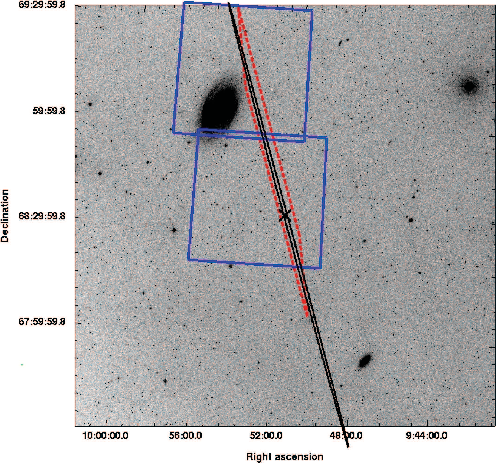
\includegraphics[scale=0.6]{m81_from_Hurley10.pdf} 
%           \end{figure}
%           \end{center}
%
%           \column{0.5\textwidth}
%           \begin{block}{Some text}
%               Goes here
%           \end{block}
%       \end{columns}
%   \end{frame}
%
%   \begin{frame}
%       \frametitle{Gamma-ray Bursts}
%
%       \begin{itemize}
%           \item GRB\,051103~\cite{2012arXiv1201.4413T}
%       \end{itemize}
%
%       \begin{columns}[]
%           \column{0.5\textwidth}
%           \begin{block}{Some text}
%               Goes here
%           \end{block}
%
%           \column{0.5\textwidth}
%           \begin{center}
%           \begin{figure}
%               \vspace*{-1.0cm}
%               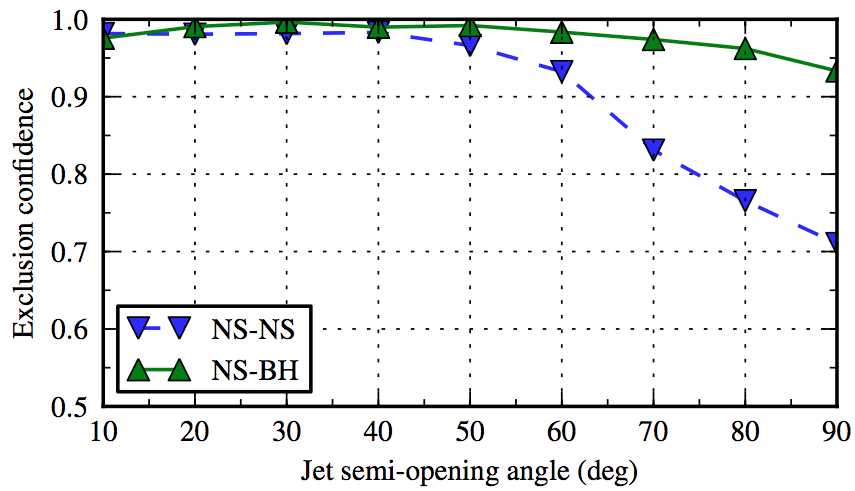
\includegraphics[scale=0.18]{jet_exc_PRODUCTION.png}  \\
%               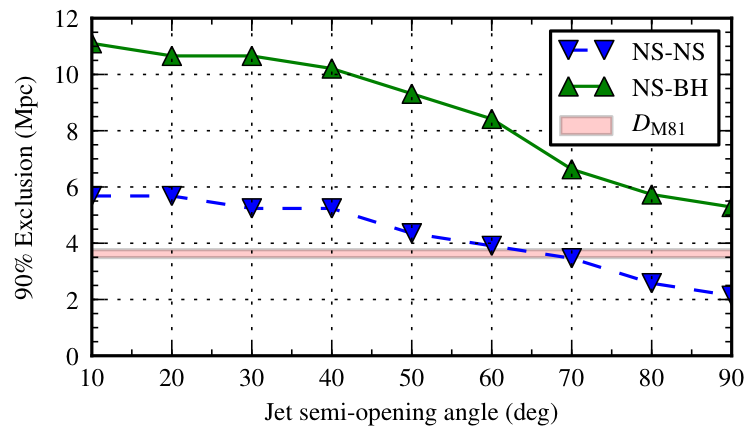
\includegraphics[scale=0.2]{D90_exc_PRODUCTION.png} 
%           \end{figure}
%           \end{center}
%       \end{columns}
%
%   \end{frame}


%\begin{frame}
%    \frametitle{Binary Black Holes}
%    \begin{itemize}
%        \item
%    \end{itemize}
%\end{frame}

%\section{Future GW Astronomy}

%\begin{frame}
%    \tableofcontents[currentsection]
%\end{frame}

%\subsection{When will we see something, what will we see?}

%\begin{frame}
%    \frametitle{Advanced LIGO}
%    When will we see something?
%    \begin{itemize}
%        \item
%    \end{itemize}
%\end{frame}

\section{Conclusion}

%   \subsection{Advanced LIGO: Observing Scenarios}
%   \begin{frame}
%       \frametitle{Advanced LIGO}
%   \end{frame}

\begin{frame}
    \frametitle{Summary}
\end{frame}

\begin{frame}[allowframebreaks]
    \frametitle{References}
    \bibliography{biblio}
\end{frame}



\end{document}
